\cleardoublepage

\chapter{Resultados}
\label{makereference7}

\section{Entrenamiento}

\section{Calidad del código}

\begin{figure}[htb]
	Una vez acabado el código del proyecto, decidimos certificar su calidad mediante \textbf{codacy}.
	\textbf{Codacy} es una herramienta que proporciona nuestro controlador de versiones \textbf{GitHub}. Sencillamente revisa todas y cada una de las líneas del código, para hacerlo más sencillo, escalable y seguro. Genera un informe con los errores y te dice qué grado de calidad tiene, siendo A el más alto.
	
	\begin{center}
		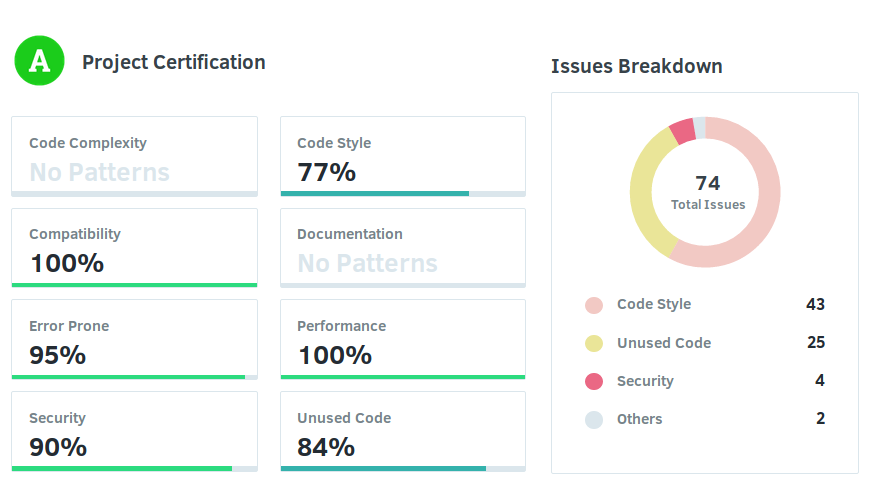
\includegraphics[height=3.5in]{figures/codacy.png}
		\caption{Informe de nuestro proyecto}
	\end{center}
	
	\label{figure7}
\end{figure}